\chapter{Background}\label{sec:background}
\section{Software Product Lines}
We will first give a brief introduction to \emph{Software Product Lines}.
More background details can be found in for example~\cite{van2001notion, apel2013software, bosch2000design}.
Software Product Lines use the same idea as age-old industrial product lines.
The idea behind them is that variants of products can be easily created when 
multiple products use the same general parts. If these parts can be created
in the same factory, we only need to combine these in different ways to create
multiple products. This idea can be read in the context of industrial
manufacturing, where we can for example create different aeroplanes that have
great overlap in their parts. We can also read this in the context of software,
this is where we talk about Software Product Lines.

Concepts used in software product lines include features, configurations,
variants and products. Since we will also use these concepts throughout this
work, let us look at them in more detail. \emph{Features} are ``\emph{a logical unit of
behaviour that is specified by a set of functional and quality requirements}'',
according to~\cite{bosch2000design}. This means that features implement the requirements
of a system, an example would be sending messages in an e-mail system. These features
can be toggled on and off, they are binary. In source code, features can be implemented
for example using \texttt{\#ifdef} statements. \emph{Configurations} can be seen as a
list of all features with all of them either enabled or disabled. Configurations can
be deemed valid with the use of \emph{Feature Models}, which describe relations between
features. One could see how features such as \emph{Linux} and \emph{Windows} should not
occur simultaneously. \emph{Variants} or \emph{products} are configurations applied to
full systems. By applying them, certain parts in the source code can be removed, whilst
others should stay, decided by the variability mechanism (i.e. the \texttt{\#ifdef} 
statements).

\section{Virtual Platform}\label{sec:background:vp}
In this section, we will go more in-depth into some specifics of the Virtual
Platform~\cite{mahmood2021}. We do this because we want to formally define
the framework. Besides that, we want to extend the framework
with two accompanying operators, which will of course be formalised in the
created formalisation. 

The Virtual Platform consists of several conceptual structures on which the
operators within it work. These structures are especially important to us as we
will formalise them in Chapter \ref{sec:vp:formalisation}. The most important
structure is the assets, making up the \emph{Asset Tree} (AT), an abstraction
of software repositories with their included assets. Assets make up
the complete structure of the software product line. They can be anything from
folders to methods. The asset tree is a hierarchical, non-cyclic tree where the 
nodes are all assets. Each asset has a specific asset type, a version, a presence
condition and a number of possible child assets. Each asset may also have a
\emph{Feature Model} (FM) attached. 
Certain asset types may only be in children of certain other asset types, for
example, we do not want a folder asset type to reside in a file asset type.
Features have names and two parameters, being \emph{optional} and
\emph{incomplete}. Optionality describes whether or not the feature is
mandatory, incompleteness describes whether the feature is fully implemented or
not. Since we want to have feature models, features can also have subfeatures. 
A feature model can then consist of just a root feature and a special
feature called ``unassigned''. This last feature can be used to mount features
resulting from clone operations which were previously not mounted in the model
at all. The Virtual Platform uses a \emph{Trace Database}, which keeps track of
clones of assets through the asset tree, this together with the versions of assets
and features can be used to propagate changes between clones.

The Virtual Platform already contains numerous operators to work on the internal
structures. The two operators we will add, work alongside the existing operators.
This means that we do not have to keep in mind how they might interact with the
internal structures. Our new operators are special in the way that they have a
necessary order in which they can be used, the \emph{put} must be used after the
\emph{get}, and the \emph{get} operator can only be used while there is no `active'
clone in progress.

For this work, the most important structures are the assets and the features.
We do not need to formalise the notion of the trace database or the versions as
our new operators will not use these. In our formalisation, we also abstract the
feature models such that they are described using an expression. This
simplifies the formalisation of features as they can then consist of just a
name.

\section{Lenses}\label{sec:background:lenses}
A lens \(l\) is a mapping between a set \(C\) of ``concrete''
structures (also called \emph{sources}) and a set \(A\) of ``abstract'' structures 
(also called \emph{views}), consisting of
three functions \emph{get}, \emph{put} and \emph{create}~\cite{foster2007}. The \emph{get}
function takes a concrete structure and yields an abstract structure. The
\emph{put} function does the reverse: it takes an abstract structure combined
with the original concrete structure and gives back a new concrete structure.
Finally, the \emph{create} function is much like the \emph{put} function, but
lacks the original concrete part. The \emph{create} function can thus create
a concrete structure from just an abstract structure. Formally, we get:
\[
  \begin{array}{lll}
    \textit{get} & : & \unaryFunc{C}{A} \\
    \textit{put} & : & \binaryFunc{A}{C}{C} \\
    \textit{create} & : & \unaryFunc{A}{C}
  \end{array}
\]
For a set of these three functions to be called a lens, they have to satisfy some
lens laws. These lens laws ensure so-called acceptability (\putget)
and stability (\getput):
\[
  \begin{array}{ll}
    \mathit{put}\left(\textit{get}~c\right)~c = c & \getput \\
    \mathit{get}\left(\textit{put}~a~c\right) = a & \putget \\
    \mathit{get}\left(\textit{create}~a\right) = a & \createget
  \end{array}
\]
How all of these definitions work together can best be seen in the form of
the schema shown in Figure~\ref{fig:lens:overview}. Here we can see two
concrete structures $s$ and $s'$, connected by the \emph{get} and \emph{put} functions.
The abstract structure $v$ is the result of applying \emph{get} to the source $s$ and $v'$
is the view that results from the edits made to $v$. We see a dashed line back
to $s$ from $v$, this represents the \getput~law. A similar dashed line can be
seen from $s'$ to $v'$, this represents the \putget~law. We of course also have
an arrow from $v'$ to $s'$, showing how to finish the loop towards the new
concrete structure.

\begin{figure}
  \centering
  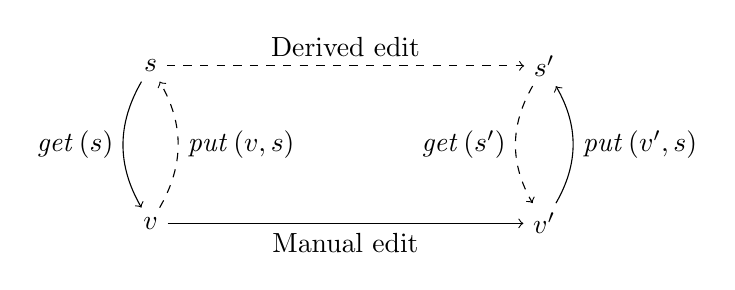
\begin{tikzpicture}
    \node[] (OS) at (0, 2) {$s$};
    \node[] (OV) at (0, 0) {$v$};
    \node[] (ES) at (5, 2) {$s'$};
    \node[] (EV) at (5, 0) {$v'$};
    
    \draw[dashed,->] (OS) -- (ES) node [midway, above] {Derived edit};
    \draw[->] (OV) -- (EV) node [midway, below] {Manual edit};
    \path[->] (OS) edge[bend left=-30] node[left] {$\mathit{get}\left(s\right)$} (OV);
    \path[dashed,->] (ES) edge[bend left=-30] node[left] {$\mathit{get}\left(s'\right)$} (EV);
    \path[dashed,->] (OV) edge[bend right=30] node[right] {$\mathit{put}\left(v, s\right)$} (OS);
    \path[->] (EV) edge[bend right=30] node[right] {$\mathit{put}\left(v', s\right)$} (ES); 
  \end{tikzpicture}
  \caption{Overview of a standard lens.}
  \label{fig:lens:overview}
\end{figure}

\section{Current State of Research}
The most closely related work to ours is by St{\u{a}}nciulescu et al., which is
a view-based editing method~\cite{stuanciulescu2016} as well. Their system is
defined in the formalisation of variational software called \emph{Choice Calculus}~\cite{walkingshaw2014}
and also uses the concept of lenses.
Choice calculus abstracts away the notation of \texttt{\#ifdef} statements into
a more formal syntax to simplify the definitions. Our work will not be 
based on choice calculus, but rather on the conceptual structures of the Virtual
Platform. We will still take a closer look at how this method works because we are
going to compare to this method in the evaluation (Section~\ref{sec:evaluation}).

Choice Calculus is a way to abstract variational source code into a more consise
format~\cite{erwig2011choice}. Figures~\ref{fig:representations:sourcecode} and 
\ref{fig:representations:choicecalculus} show how a piece of variational source
code is represented using choice calculus. In the first subfigure, we see the source
code, where \texttt{a} is guarded by the feature \texttt{F}. If \texttt{F} does not
hold, then we want \texttt{b} to be active. In the second subfigure we see this
represented in the choice calculus. We again see the feature $F$ and the codes $a$
and $b$. The representation means that if $F$ is true, we pick $a$, otherwise we
pick $b$. If an \texttt{\#ifdef} does not contain an \texttt{\#else} statement,
the second argument of the choice can be replaced by an empty line of code. For
example, removing the \emph{else} clause from our example would give us \(\mathit{F}\!\left<a, \iota\right>\).
The $b$ line is now removed and replaced by \(\iota\). 

\begin{figure}
  \centering
  \begin{subfigure}[b]{0.4\textwidth}
    \centering
    \begin{BVerbatim}
#ifdef F
  a
#else
  b
#endif
    \end{BVerbatim}
    \caption{Source code}
    \label{fig:representations:sourcecode}
  \end{subfigure}
  \hfill
  \begin{subfigure}[b]{0.4\textwidth}
    \centering
    \(\mathit{F}\!\left<a,b\right>\)
    \caption{Choice calculus}
    \label{fig:representations:choicecalculus}
  \end{subfigure}
  \caption{Different representations of variational source code.}
  \label{fig:representations}
\end{figure}

In the previous work which was also based on lenses, the \emph{get} operator 
requires a \emph{choice}. With this \emph{choice}, the programmer determines 
the set of variants included in the view (expressed in terms of activated and
deactivated features). In our example of Figure~\ref{fig:representations:choicecalculus},
a choice of $F$ would yield just $a$, instead of the full choice. The negation of
$F$ (\(\neg\mathit{F}\)) would give just $b$. If $F$ is not decided on by the choice,
the choice block remains in full.

The \emph{put} operator requires another expression, called the \emph{ambition}.
The ambition is a way for the programmer to determine the set of variants to
which the changes should be applied. The way the \emph{put} operator deals with
this ambition, is by creating a new top-level choice (a representation of an
\texttt{\#ifdef}) in the form of \( \left(c \land a\right)\!\left<v', s\right> \).
Here, $c$ and $a$ are the chosen choice and ambition in the \emph{get} and
\emph{put} operators, $v'$ is the edited view and $s$ is the source from which
the view originated. This top-level choice is then minimised such that the
common parts are extracted from both branches. Let us take for example the choice
calculus expression from Figure~\ref{fig:representations:choicecalculus} and apply
the \emph{get} operator with as choice $F$. We already know this results in just $a$
as the source code. We as the programmer now decide to change this to $c$. To push
these changes back into the original source code, we use the \emph{put} operator.
As the ambition, we again choose $F$, resulting in the choice calculus expression of
\(\mathit{\left(F \land F\right)}\!\left<c,\mathit{F}\!\left<a,b\right>\right>\).
We can simplify this expression in two ways: firstly, we can simplify the first 
choice expression by replacing \(\mathit{F} \land \mathit{F}\) to just \(\mathit{F}\).
Secondly, we can replace the \(\mathit{F}\!\left<a,b\right>\) by $b$, since we know
that $F$ does not hold in this part of the first choice level.

The limitations of the previous work, as mentioned before, are twofold. Firstly, the
method is not proven to be correct with the lens laws. This means that we cannot strictly
say that the method uses lenses. More importantly, we cannot ensure the round-tripping
properties that lenses want to ensure. Moreover, we will later give a counterexample
that disproves one of the lens laws for the previous work. The second limitation of the
previous work is the way the \emph{put}
operator works. It does not allow changes to be propagated to a scope beyond
the \emph{choice} expression from the \emph{get} operator. This was a
deliberate design choice as it holds to the \emph{Edit Isolation Principle},
where changes can only be made to what is visible in the view. To see how this works,
let us look at Figure~\ref{fig:representations:sourcecode}. If we create a view with
only feature \texttt{F}, we result in a view with just \texttt{a}. Now the \emph{Edit Isolation Principle}
says that we cannot make any edits such that any of the left out code can be changed.
In this case this means that we cannot make changes to the code in \texttt{b}. 
This work aims to lift the above two limitations, we want to create a method in which
the \emph{Edit Isolation Principle} is lifted and for which we can prove the lens laws.

\section{Running Example}\label{sec:background:example}
In this work, we will generally use the sample example system to show the workings of
the formalisations. This is a simple application that initially has three classes
embedded in one file. Our system has two features, namely an optional \emph{CLI} and
\emph{logging}. We have that \emph{logging} can only be enabled when \emph{CLI} is
enabled, guarded by a feature model. In the end, we want to be able for a developer
to work only on a part of the file, and then be able to also push these changes
back into the full source file.

An example of how this source code might look can be found in Figure~\ref{fig:runningexample}.
We first what the entire source code looks like in Figure~\ref{fig:example:original}.
As explained before, we have one base class that is not locked behind a feature and two
classes that are locked behind the \emph{CLI} and \emph{logging} feature, respectively.
To show why projectional editing can be beneficial, see Figure~\ref{fig:example:view}.
In this view we have left out the \emph{logging} feature and have selected the \emph{CLI}
feature. We can see this, as the \emph{CLI} feature is not surrounded by \texttt{\#ifdef}
statements, and the \emph{logging} feature is left out altogether. The view is easier to
edit for a developer, as there is fewer code. The benefits seem marginal here, but one
can imagine that within the classes \texttt{Base} and \texttt{CLI}, there might be specific
code for the other features as well, which would also become less complex in the view.

\begin{figure}
  \centering
  \begin{subfigure}[b]{0.45\textwidth}
    \centering
    \begin{BVerbatim}
public class Base
{
  ...
}

#ifdef CLI
public class CLI
{
  ...
}
#endif

#ifdef logging
public class logging
{
  ...
}
#endif
    \end{BVerbatim}
    \caption{Original example source code.}
    \label{fig:example:original}
  \end{subfigure}
  \hfill
  \begin{subfigure}[b]{0.45\textwidth}
    \centering
    \begin{BVerbatim}
public class Base
{
  ...
}

public class CLI
{
  ...
}
    \end{BVerbatim}
    \caption{Example view of example source code.}
    \label{fig:example:view}
  \end{subfigure}
  \caption{Running example source code.}
  \label{fig:runningexample}
\end{figure}
